\documentclass[10pt]{article}
\usepackage{W266FinalProject}
\usepackage{times}
\usepackage{url}
\usepackage{latexsym}
\usepackage{appendix}
\usepackage{graphicx}
\usepackage{amsmath}
\newcommand{\comment}[1]{}
\usepackage{graphicx}
\usepackage{booktabs}
\usepackage{subcaption}
\usepackage{fancyvrb}
\usepackage{lipsum}
\usepackage{pbox}
\newcommand{\verbatimfont}[1]{\renewcommand{\verbatim@font}{\ttfamily#1}}
\newcommand*\justify{%
  \fontdimen2\font=0.4em% interword space
  \fontdimen3\font=0.2em% interword stretch
  \fontdimen4\font=0.1em% interword shrink
  \fontdimen7\font=0.1em% extra space
  \hyphenchar\font=`\-% allowing hyphenation
}
%\usepackage{subfig}
%\usepackage{subfigure}
%\setlength\titlebox{5}

\title{An Integrated Visio-Textual Approach to Movie Genre Classification}
\author{
        Sartaj Singh Baveja \\
        UC Berkeley School of Information \\
        {\tt sartaj.baveja@berkeley.edu} \\\And
        Karthik Srinivasan \\
        UC Berkeley School of Information \\
        {\tt kasri@berkeley.edu} \\
        % \\[-3.0ex]
}

\begin{document}
\maketitle

% \vspace*{-1cm}

% Abstract
\begin{abstract}
As movie collections within streaming services grow, providing relevant movie recommendations have become increasingly important for customer satisfaction and retention. For this purpose, classification of movies into genres have taken center stage. In this paper, we describe a novel method of combining the movie plot summaries with their poster publications to better predict its genre. We propose a multi-headed deep neural network (DNN) that simultaneously train the plot summaries and poster images, while maximizing $F_1$ scores. We show that the results from this integrated DNN out-perform conventional Natural Language Processing (NLP) and convolutional networks (CNN).  
\end{abstract}

% Section : Introduction
\section{Introduction}
\label{intro}
The film industry is going through a massive shift in the way customers are consuming their products. In particular, streaming movie services such as Netflix, Amazon Prime, Hulu, and Disney have become the go-to medium for movie consumption. Rising competition within streaming service companies have led to a shift in focus towards customer satisfaction and retention. To ensure high customer engagement on their platforms, it is not merely enough to accumulate a large repository of content. Instead, streaming services have invested heavily in refining their search and recommendation engines~\cite{NetflixChallenge} for increased customer engagement.

Genre of a movie is predominantly used to help refine search and recommendations. The task of labeling movies with genres, mostly carried out by humans, results in subjective errors and an inability to capture varying proportions of each genre. For example, a movie could be mostly Action with an element of Comedy, an aspect that is not captured through existing human labeling methodologies. However, having an automated genre labeling system could adequately capture nuances of a movie through genre prediction probabilities.

Machine learning has played a vital part in the automation of genre labeling. The earliest attempts focused on examining the audio-visual content (\cite{Nam1998}, \cite{Rasheed2002}) through low-level audio-visual features. More advanced deep learning techniques were later introduced~\cite{WEHRMANN2017973} that improved performance multi-fold. However, availability of trailers for movies of all languages and eras poses a significant challenge for the widespread adoption of this method. Instead, researchers have now turned to the use of movie plots and movie posters to overcome the ``availability" challenge. 

Our current work aims to integrate the information available through posters and movie plots to generate more accurate genre labels. To the best of our knowledge, there has been no previous work that combines movie posters and plot summaries for genre classification. In this paper, we demonstrate the benefits of the aforementioned integrated deep learning model, and compare with state-of-the-art NLP algorithms.

% Section : Literature Survey
\section{Literature Survey}
There have been extensive studies on movie genre classification through conventional machine learning (ML) and deep learning techniques. Researchers have attempted to tackle the multi-label classification problem through computer vision (CV) and NLP techniques. In this section, we review previous work addressing genre classification of movies through CV and NLP methods.

% Sub Section : Posters
\subsection{Classification using Posters}
\label{sec:LitPosters}
Researchers from Georgia~\cite{ZhouHermans2010} showed that scene categorization of movie trailer keyframes performed significantly better than using low-level visual features such as average shot length, color variance, key lighting, and motion content. They constructed a bag of visual words model from the extracted keyframes, and represent each trailer as a temporally segmented 2D histogram of scene categories subsequently used in similarity scores. In 2015, researchers~\cite{IvasicPobar2014} extracted visual and structural features from poster images, subsequently used in distance measures for classification through nearest neighbour techniques.
A new study~\cite{wi2020} augmented state-of-the-art convolutional neural networks, such as ResNet~\cite{HeZRS15}, with a Gram layer that extracts optimal information and characteristics from movie posters resulting in an $F_1$ score increase of $\approx 1\%$. 

% Sub Section : BERT
\subsection{Classification using Plot Summaries}
With an increase in the capabilities of NLP, interest in movie genre classification using plot summaries has been renewed. Until recently, genre classification was predominantly used for information retrieval. Researchers~\cite{Goldstein2007} used combination of layouts, characters and other structural features to classify genres using traditional ML techniques ( Random Forest, SVM and Naive Bayes). As the availability of data and compute power grew, advanced deep learning techniques, such as Gated Recurrent Units~\cite{hoang2018predicting}, were successfully used for movie genre classification. More recently, Bi-directional LSTM~\cite{Ertugrul2018} networks trained on Word2Vec~\cite{mikolov2013efficient} embeddings were found to perform better on individual sentences of the plot summary than in its entirety.

Inspired by the previous success of using posters and plot summaries, as discussed above, we propose a novel method to combine both posters and plot summaries. The rest of this paper describes the data, the proposed models, their performance and the challenges associated.

% Section : Data Mining and Exploration 
\section{Data Mining and Exploration}

% Sub Section : Data Mining
\subsection{Data Mining}
We use IMDB to collect movie genres, posters and plot summaries, and scale data extraction tasks through AWS serverless lambdas. A pre-trained CNN model generates the feature vectors for the posters. Subsequently, we merge these feature vectors with the original data. Finally, we divide our dataset into a train, development and validation sets (60/20/20 split).

% Sub Section : Data Exploration
\subsection{Data Exploration}
\label{sec:DataExploration}
The dataset contains 81,271 records with 27 unique genres. Due to sparsity of data across various genres, we choose to restrict our analysis to the ten most common genres. Drama, Comedy and Romance are the most frequently occurring genres, present in more than 60\% of the records. Upon closer examination of plot summary length distributions, we observe long tails and choose to filter out summaries $>545$ words (the upper $1\%$ tail). On the other end, we also filter out plot summaries of shorter length ($<15$ words, the lower $1\%$ tail). We also observe that movies in our dataset span between years 1906 and 2020, with majority of the movies between 2010 and 2020. The dataset contains 154 unique movie languages with over 50\% of those in English. The count of movies in each genre, depicted in Figure~\ref{fig:genrehist}, highlight the imbalance in our dataset.

\vspace{2.0mm}
\begin{figure}[!h]
  \centering
  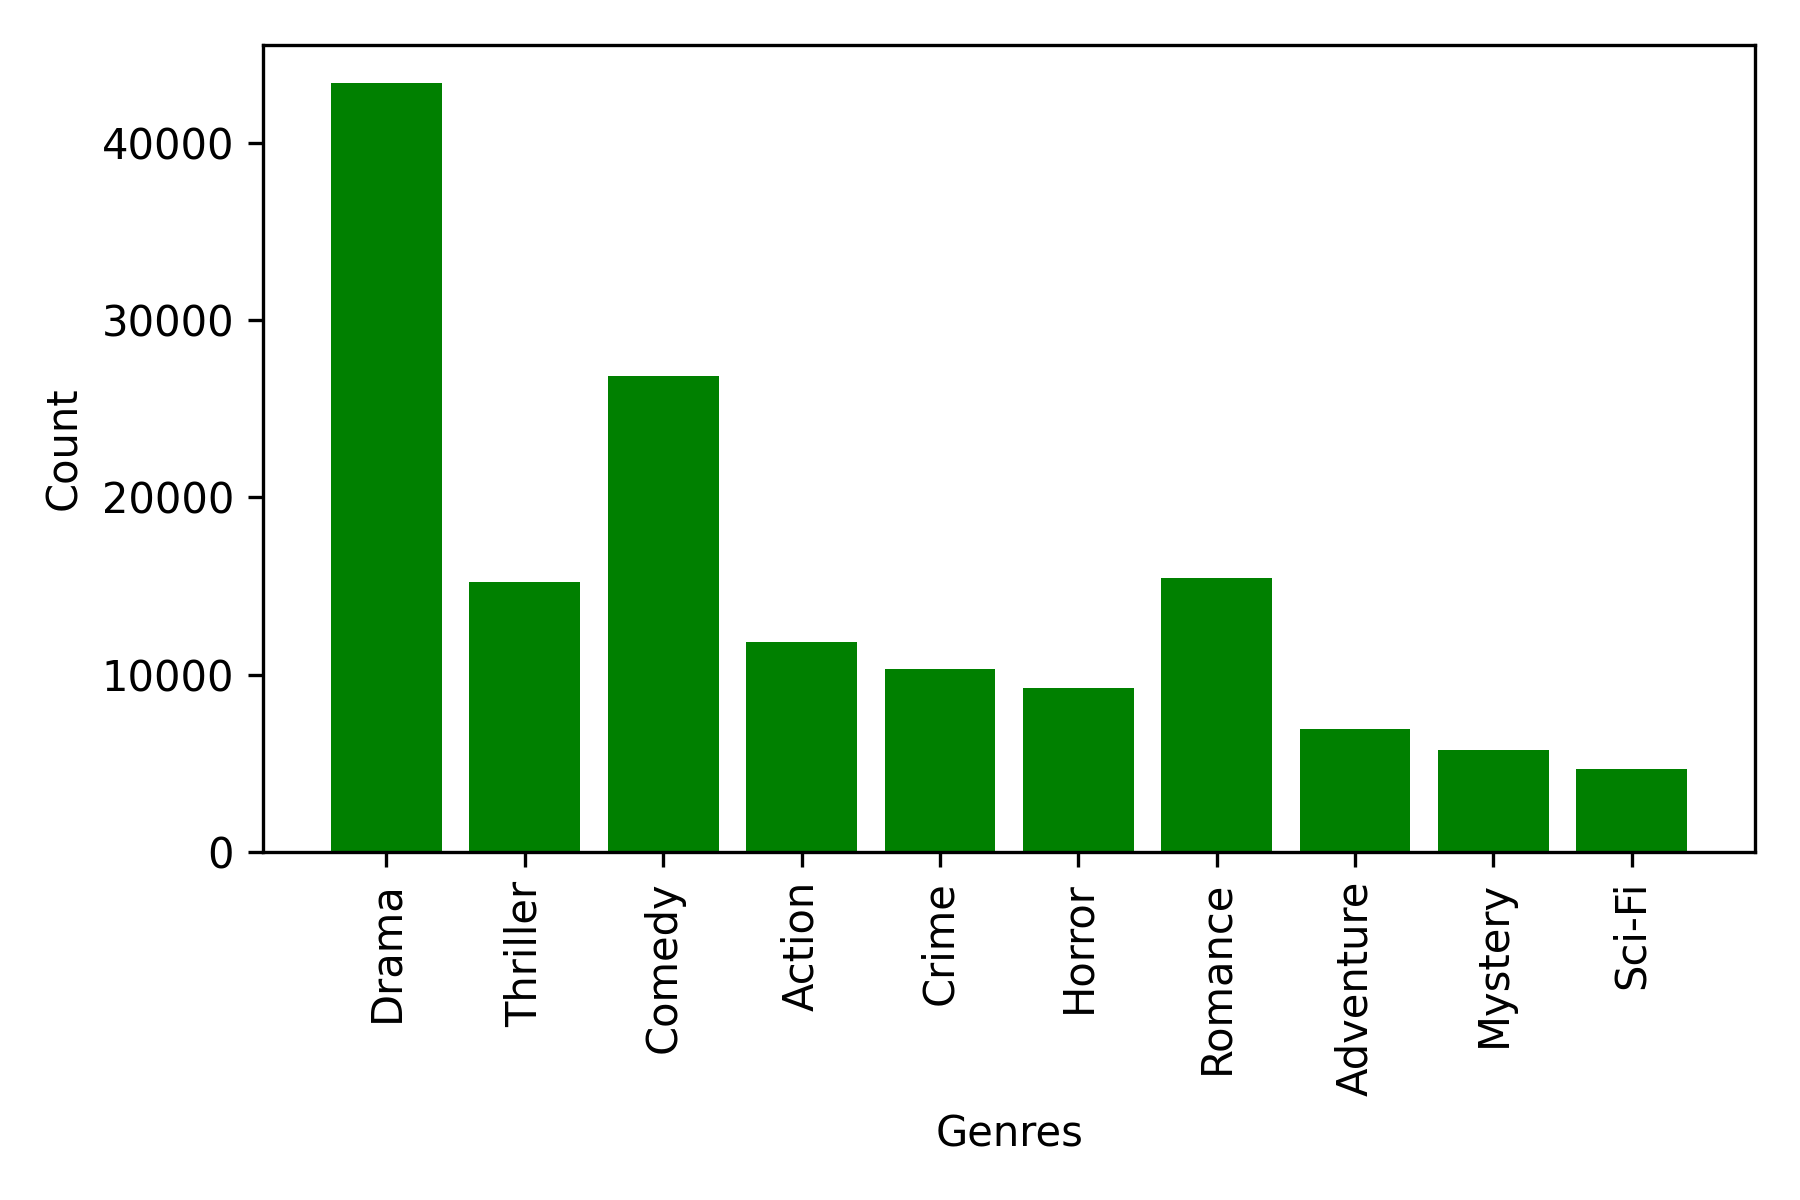
\includegraphics[width=0.5\textwidth]{images/GenreCount.png}
  \caption{Number of movies per genre.}
  \label{fig:genrehist}
\end{figure}

% Section : Modeling Methodology
\section{Modeling Methodology}

In this section, we describe the baseline, state-of-the-art and our proposed integrated visio-textual model. In all of the models described below (other than the naive most common class classifier), we use pre-trained models as a starting point and fine tune the weights as appropriate. However, we make no changes to the underlying architecture of the pre-trained models.

% Sub Section : Most Common Class
\subsection{Model 0: Most Common Class}
For this model, we consider the most common class within each genre label to be the baseline. In the train dataset, only the Drama genre label is available on $>50\%$ of the dataset and is hence chosen as the default class. The rest of the genre labels do not fall in the majority class and are therefore not chosen. This implies that we predict every plot summary/poster combination will be predicted as Drama. In Table \ref{F1Table}, we tabulate the weighted F1 score of such a prediction, and this is the minimum score to improve upon for any ML classifier. 

% Sub Section : CNN
\subsection{Model I: Convolutional Neural Network: Posters}
As discussed in Section \ref{sec:LitPosters}, prior work demonstrated the possible use of poster images to predict the genre labels. In this work, we use pre-trained Resnet50~\cite{HeZRS15} to generate feature vectors for the poster images of dimensions (224, 224, 3). These feature vectors, each of dimension 2048 are directly input into an affine layer with a sigmoid activation that generate predictions for the genre labels (see Figure~\ref{fig:poster}).

\begin{figure}[!htb]
    \centering
    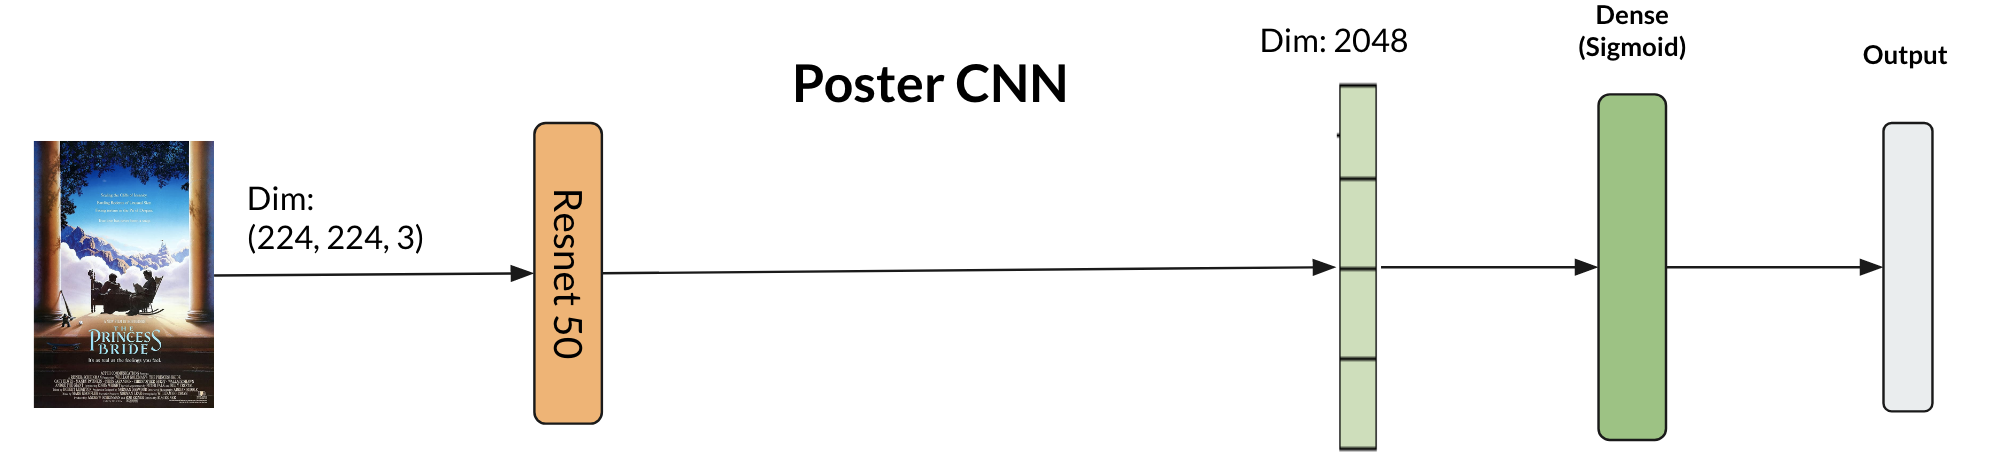
\includegraphics[width=0.5\textwidth]{images/Poster.png}
    \caption{CNN architecture for poster images.}
    \label{fig:poster}
\end{figure}

% Sub Section : BERT
\subsection{Model II: Bidirectional Encoder Representations from Transformers (BERT): Plot Summaries}
We construct the main baseline for this work where plot summaries are input into a BERT model \cite{DevlinBERT} fitted with a classification head, as shown in Figure~\ref{fig:bert}. To limit train costs and time, we initialize the weights using a pre-trained~\cite{turc2019} 12-layer, 768-dimensional hidden vector, uncased model. We tokenize these plot summaries into a BERT-friendly format and subsequently trim them to a maximum length of 128 tokens. This then connects to two fully connected layers followed by an affine transform with sigmoid activation resulting in probabilities for label predictions. For our BERT baseline, we consider two cases where, (i) we use the pre-trained model with no fine tuning, and (ii) we fine-tune all the layers of the model.

\begin{figure}[!htb]
    \centering
    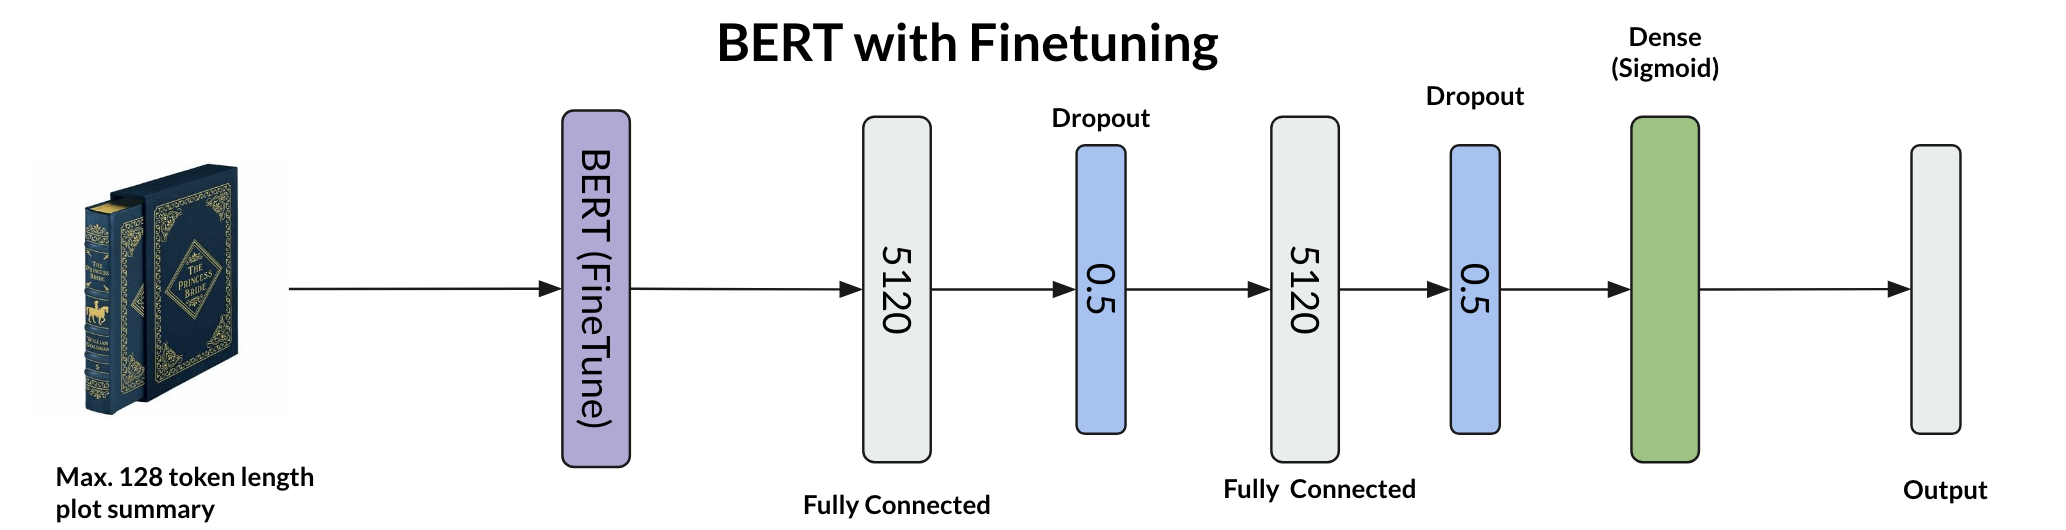
\includegraphics[width=0.5\textwidth]{images/BERT-DNN.png}
    \caption{BERT DNN architecture for plot summaries.}
    \label{fig:bert}
\end{figure}

% Sub Section : Integrated BERT and ANN
\subsection{Model III: Integrated BERT and Poster CNN}
For our integrated model, we combine the architectures from our Poster CNN model and the fine-tuned BERT model. A concatenation layer combines the information from both models by merging the poster feature vectors (of dimension 2048) with the output from fully connected layers of the BERT model (of dimension 5120) resulting in an output layer of dimension 7168. This concatenated vector passes through a fully connected layer and an affine layer with sigmoid activation.

\begin{figure}[!h]
    \centering
    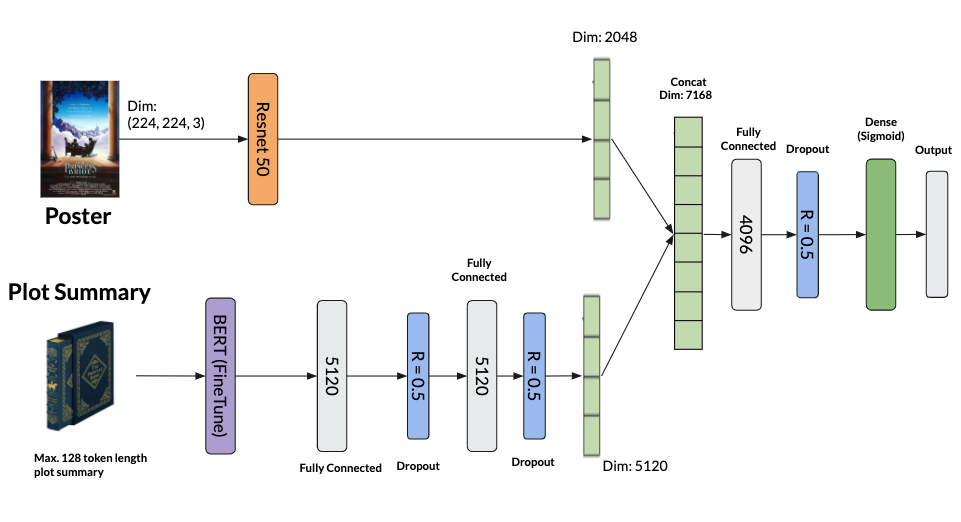
\includegraphics[width=0.5\textwidth]{images/Combined.png}
    \caption{Multi-headed deep learning architecture for combined plots/posters inputs}
    \label{fig:combined_arch}
\end{figure}

% Section : Results
\section{Results}
In this section, we compare the performance of our integrated model with the baseline models. We discuss the construction of our custom loss function and analyze the model predictions by inspecting a few examples.

% Sub Section : Accuracy Metrics and Loss Functions
\subsection{Accuracy Metrics and Loss Functions}
We use weighted $macro-F_1$ score, computed on the hold-out validation dataset, to evaluate the accuracy of the models. To begin with, the $F_1$ score for any given label $i$ is given by:
\begin{equation}
    macro\;F_{1,i} = \frac{2\cdot TP_i}{2\cdot TP_i + FN_i + FP_i + \epsilon}
\end{equation}
where $TP_i$, $FN_i$, and $FP_i$ are true-positives, false-negatives and false-positives for the $i^{th}$ label, respectively. We also add a small perturbation $\epsilon$ (=1e-16) that stabilize the computation on edge cases. The overall weighted $F_1$ score is then,
\begin{equation}
    Wtd\;F_1 = \frac{\sum_{i=1}^{N} Freq_i\;  \cdot macro\;{F_1,i}}{\sum_{i=1}^{N} Freq_i}
\end{equation}
where $N$ is the number of labels, $Freq_i$ is the frequency of label $i$ in the validation set. Note that for a multi-label dataset, the frequencies do not require to sum up to 1.

In this work, we use a macro soft F1 loss function in lieu of the traditional binary cross-entropy losses. This choice of loss function helps optimize for the accuracy in a direct manner \cite{lipton2014thresholding}. Just maximizing macro soft F1 loss function may result in the default prediction of all positive examples. This can be avoided by adding a component to the loss function that drives it in the other direction. By doing so, we can expect the system to counter-balance its previous behaviour by generating not only positive predictions but also negative predictions in order to optimize this new loss. The modified macro soft $F_1$ loss function is,
\begin{multline}
    Loss_i = 1 \\
         - 0.5 \left(\frac{2\cdot TP_i}{2\cdot TP_i + FN_i + FP_i + \epsilon}\right) \\
         - 0.5 \left(\frac{2\cdot TN_i}{2\cdot TN_i + FN_i + FP_i + \epsilon}\right) 
\end{multline}
and,
\begin{equation}
    Total\;Loss = \frac{1}{N}\sum_{i=1,N} Loss_i
\end{equation}

% Sub Section : Hyperparameter Tuning
\subsection{Hyperparameter Tuning}

We tune various hyperparameters to maximize $F_1$ scores discussed above. With the right choice of hyperparameters, the models train within $20-30$ epochs. The finalized hyperparameters and the choices tested are listed in Table~\ref{HyperparameterTable}. 

\begin{table}[h]
\begin{center}
\begin{tabular}{ccc}
\hline \bf Parameter & \bf Final Value  & \bf Choices  \\  
\hline
Learning Rate & 1e-04 &  1e-06 $\rightarrow$ 1e-02 \\
Optimizer & ADAM & ADAM \\
 & & ADAGRAD \\
 & & SGD \\
 & & ADAMAX \\
Dropout Rate & 0.5 & 0.1$\rightarrow$0.5 \\
L2 Reg. & 0.0001 & 0.0001 $\rightarrow$0.01 \\
Kernel Initializer & Xavier &  Xavier \\
& & Rand. Normal \\
& & Rand. Uniform \\
\hline
\end{tabular}
\end{center}
\captionsetup{justification=centering}
\caption{\label{HyperparameterTable} Hyperparameters for the DNN models. }
\end{table}

% Sub Section : Model Performance
\subsection{Model Performance}

\subsubsection{Oversampling}
We reduce the label imbalances in our dataset through oversampling. We oversample six of the least-occurring genres to augment the train dataset, thereby adding an additional 30,000 records. The frequency of labels in the train dataset, with and without oversampling, along with the validation set is shown in Table~\ref{FreqTable}. Please note that the oversampling is only carried out on the train dataset which is much more balanced now. 

\begin{table}[h]
\begin{center}
\begin{tabular}{cccc}
\hline \bf Label & \bf Train  & \bf Train  & \bf Validation \\  
& OS & No OS & \\
\hline
Drama & 0.49 &  0.55 & 0.56  \\
Comedy & 0.14 & 0.34 & 0.34\\
Romance & 0.27 & 0.20 & 0.20  \\
Thriller & 0.19 & 0.20 & 0.19 \\
Action & 0.16 &  0.15 & 0.15 \\
Crime & 0.15 & 0.13 & 0.13 \\
Horror & 0.30 & 0.12 & 0.12  \\
Adventure &  0.24 & 0.09 & 0.09  \\
Mystery & 0.16 &  0.07 & 0.08  \\
Sci-Fi & 0.20 & 0.06 & 0.06  \\
\hline
\end{tabular}
\end{center}
\captionsetup{justification=centering}
\caption{\label{FreqTable} Frequency of labels with and without oversampling (OS). }
\end{table}

\subsubsection{Weighted $F_1$ Scores}
The models' weighted $F_1$ scores on the validation set are shown in Table~\ref{F1Table}, with and without oversampling, respectively. We observe that the integrated model with oversampling performs best, with a weighted $F_1$ score of 0.453, a 2\% improvement over baseline BERT with fine-tuning.

\begin{table}[h]
\begin{center}
\begin{tabular}{ccc}
\hline \bf Model & \bf No OS  & \bf OS \\ \hline
Naive Classifier & 0.209 & - \\
Poster CNN & 0.232 & 0.210 \\
BERT & 0.192 & 0.214  \\
BERT + FineTuning & 0.433 & 0.431\\
Integrated model & 0.429 & \bf 0.453 \\
\hline
\end{tabular}
\end{center}
\caption{\label{F1Table} Weighted $F_1$ scores. }
\end{table}

The naive classifier performs poorly as expected, since every plot summary and poster combination is always predicted as Drama. We also observe that the BERT baseline model without fine-tuning does not learn on five of the minority classes. We hypothesize that a lack of substantial train data and context causes significant generalization difficulties. 

We compare genre-level predictions for the oversampled models in Table~\ref{F1Compare}. The baseline BERT model with fine-tuning performs similar to the integrated model. However, as we discuss in~\ref{sec:cooccur} below, the overall scores mask the subtle differences in model behaviors.

\begin{table}[h]
\begin{center}
\begin{tabular}{ccc}
\hline \bf Label & \bf BERT+FineTuning  & \bf Integrated  \\
\hline
Drama & 0.37 &  0.39  \\
Comedy & 0.17 & 0.16\\
Romance & 0.08 & 0.08  \\
Thriller & 0.06 & 0.07 \\
Action & 0.04 & 0.04 \\
Crime & 0.02 & 0.03 \\
Horror & 0.04 & 0.04  \\
Adventure &  0.02 & 0.02  \\
Mystery & 0.02  & 0.01  \\
Sci-Fi & 0.02 & 0.02  \\
\hline
\end{tabular}
\end{center}
\captionsetup{justification=centering}
\caption{\label{F1Compare} Weighted F1 scores for each label in the validation dataset. }
\end{table}

% Sub Section : Error Analysis
\subsection{Error Analysis}

\subsubsection{Co-occurrence Matrices}
\label{sec:cooccur}
We use co-occurrence matrices to examine the model performances. Figure~\ref{fig:cooccur} displays the co-occurrence matrix for the ground truth labels for each genre, where Drama, Comedy and Romance have much higher overlap than the rest. Alternately, the overlap across Action, Crime, Horror, Adventure, Mystery and Sci-Fi is minimal. This is noteworthy since the predictive models (\ref{fig:bert_cooccurence} and~\ref{fig:combined_cooccurrence}) are unable to replicate this behavior. While we observe that Drama, Romance and Comedy co-occur quite often in our models, the models do not perform as well for the other labels. In particular, we observe that the BERT model predicts certain genre groups together with no discriminative power to differentiate them. Consequently, it is unable to distinguish between Action, Crime, Horror, Adventure, Mystery and Sci-Fi. On the other hand, the integrated model shows better capability in predicting these genres. We attribute this benefit to the patterns/features captured through the poster inputs. Furthermore, we observe that the models, used in this study, only predict between 9 (BERT) and 14 (Integrated) unique combinations of labels while more than 400 exist. This likely indicates that the sparsity in the dataset is one of the main contributing factors to model performance.

\begin{figure}[!h]
\centering
    \begin{subfigure}[l]{0.5\textwidth}
      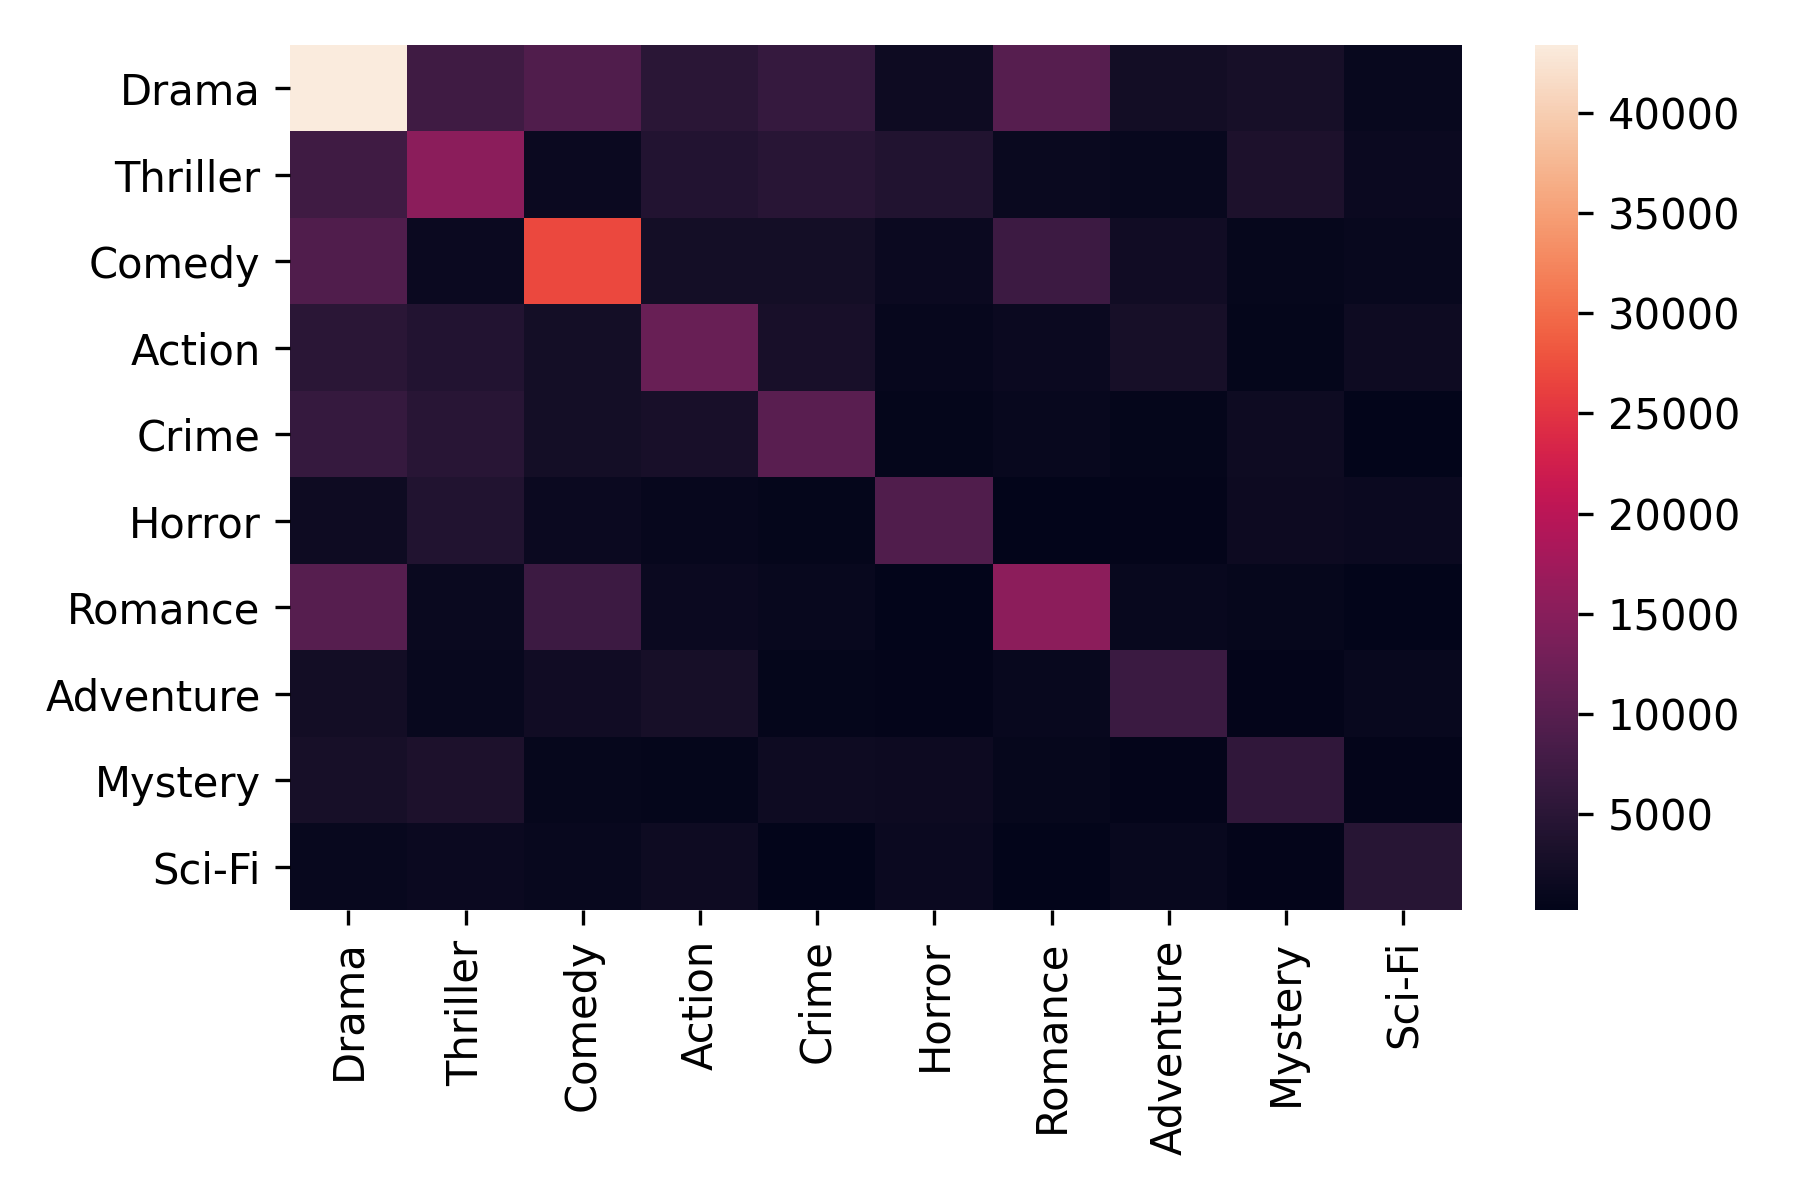
\includegraphics[width=0.95\textwidth]{images/originalCoOccurrence.png}
      \caption{Ground truth Co-occurrence Matrix}
      \label{fig:cooccur}
    \end{subfigure}
    \begin{subfigure}[l]{0.5\textwidth}
        \centering
        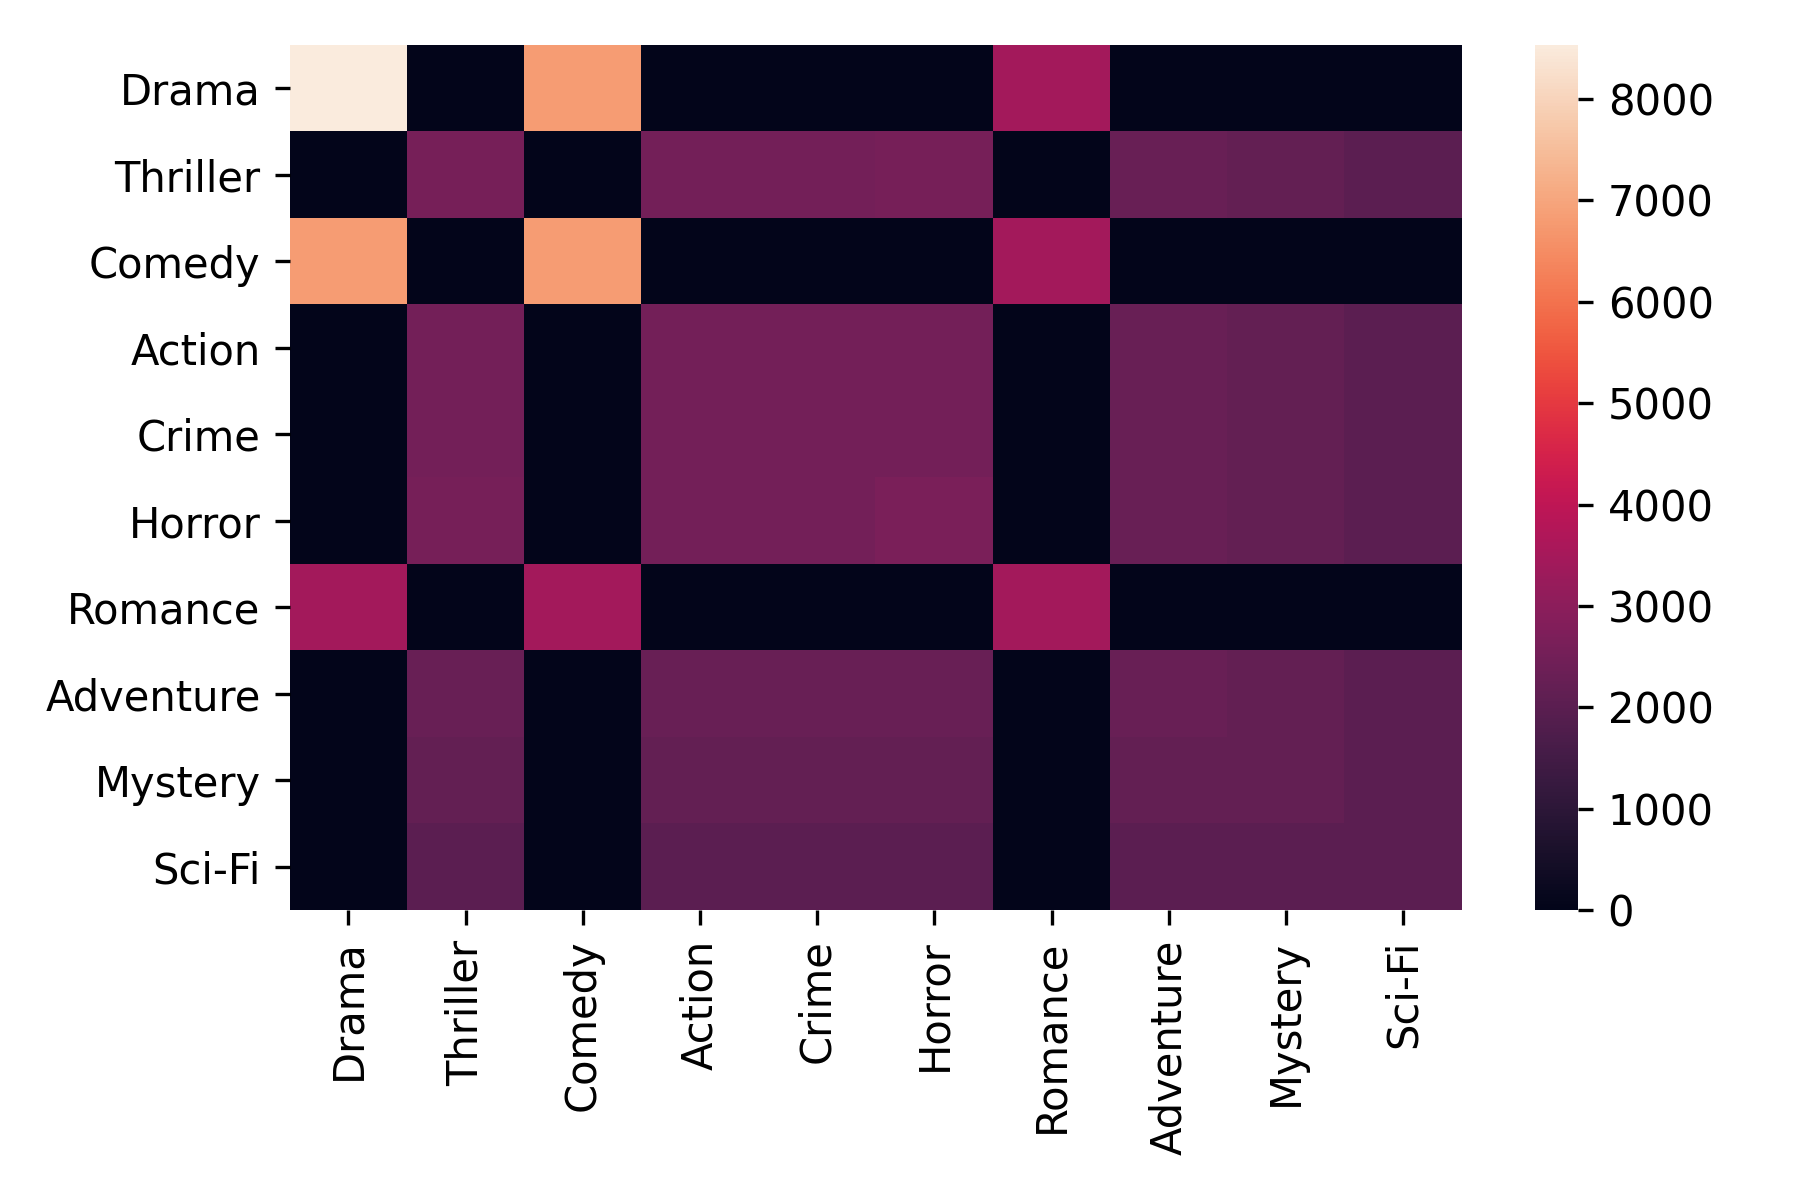
\includegraphics[width=0.95\textwidth]{images/bertCoOccurrence.png}
        \caption{Baseline BERT Co-occurrence Matrix}
        \label{fig:bert_cooccurence}
    \end{subfigure}
%\end{figure}
%    \hfill
%\begin{figure}
    \begin{subfigure}[l]{0.5\textwidth}
        \centering
        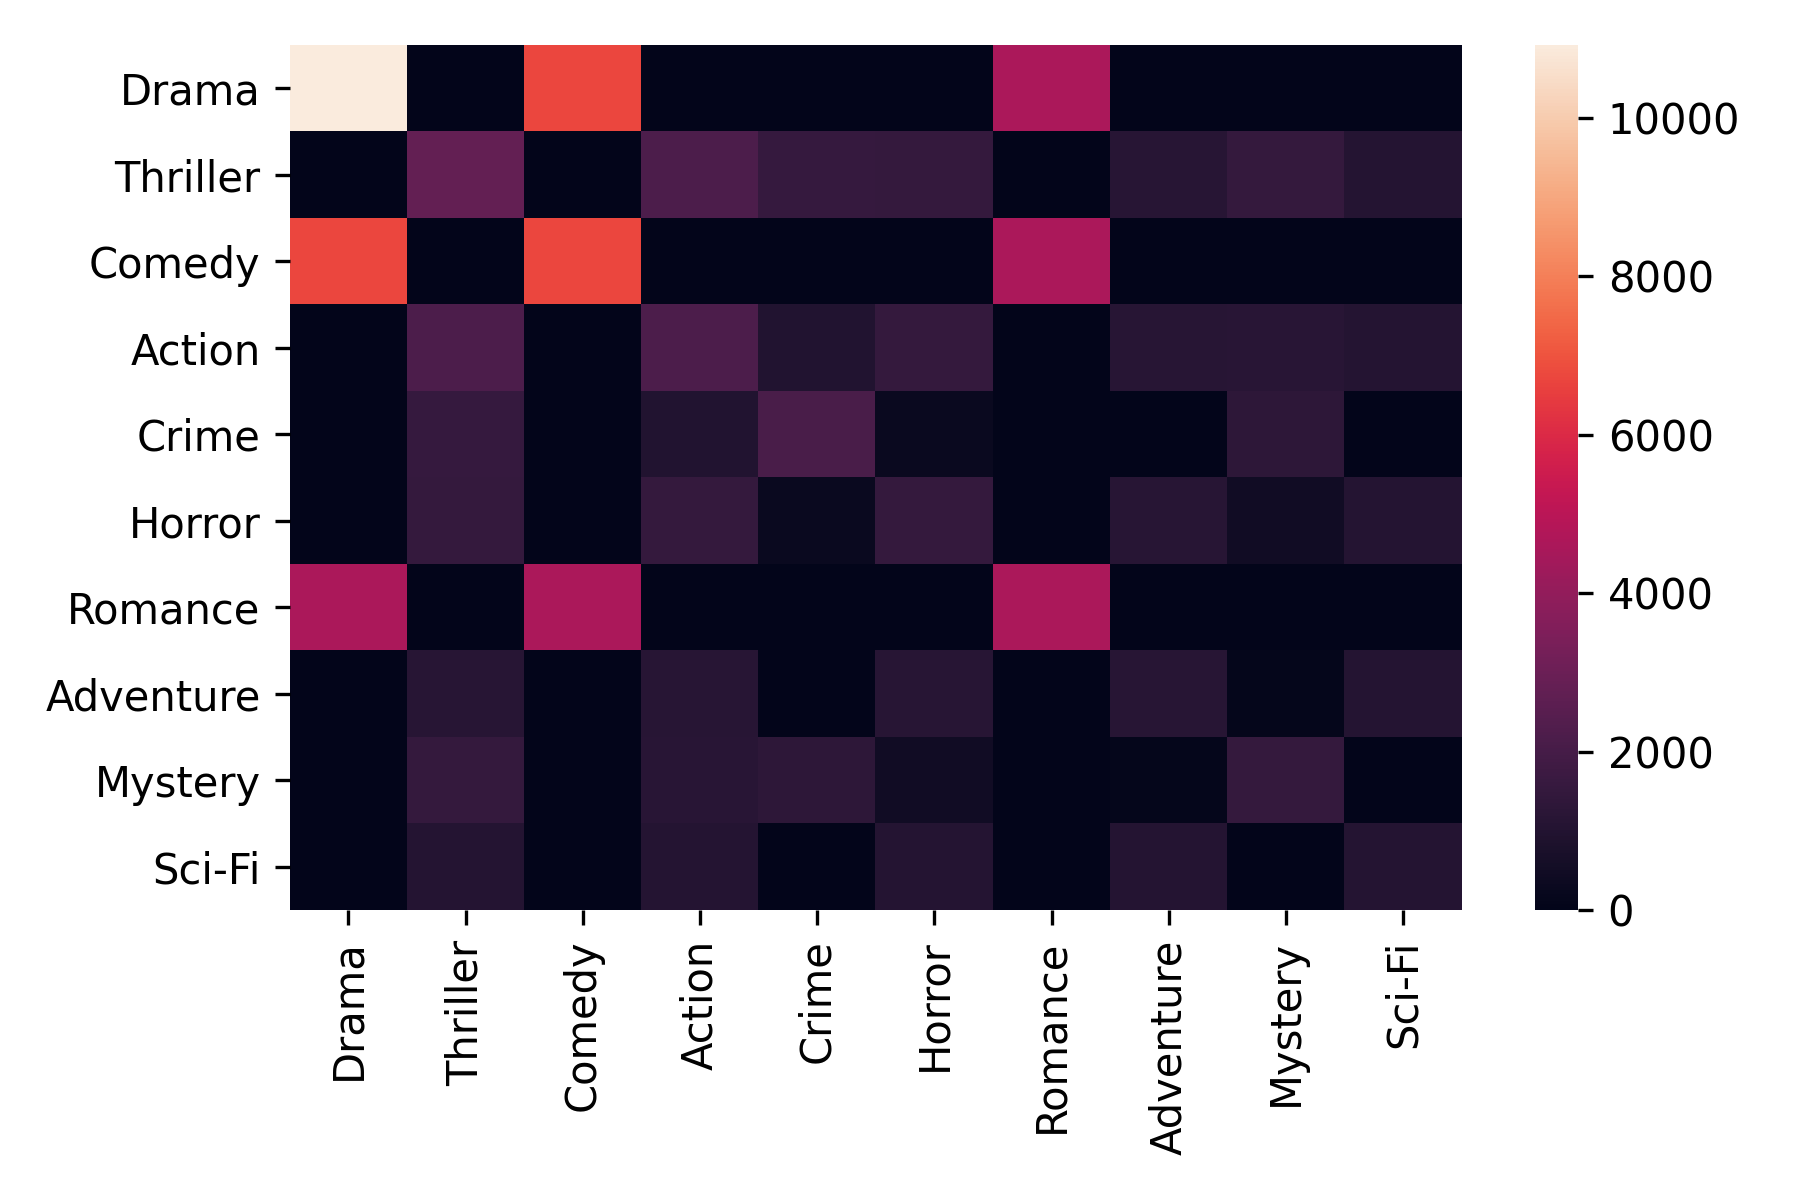
\includegraphics[width=0.95\textwidth]{images/combinedCoOccurrence.png}
        \caption{Integrated Model Co-occurrence Matrix}
        \label{fig:combined_cooccurrence}
    \end{subfigure}
\caption{Co-occurrence matrix for BERT and Integrated models.}
\label{fig:coccurrence_models}
\end{figure}

We also observe that the models overwhelmingly predict Drama whenever they predict Comedy. However, as shown in Figure~\ref{fig:cooccur}, the ground truth data suggest that a large fraction of movies are independently categorized as either Drama or Comedy, and not necessarily both. Appendix A shows a few examples of posters, plot summaries and their predictions.

\begin{figure}[!h]
    \centering
    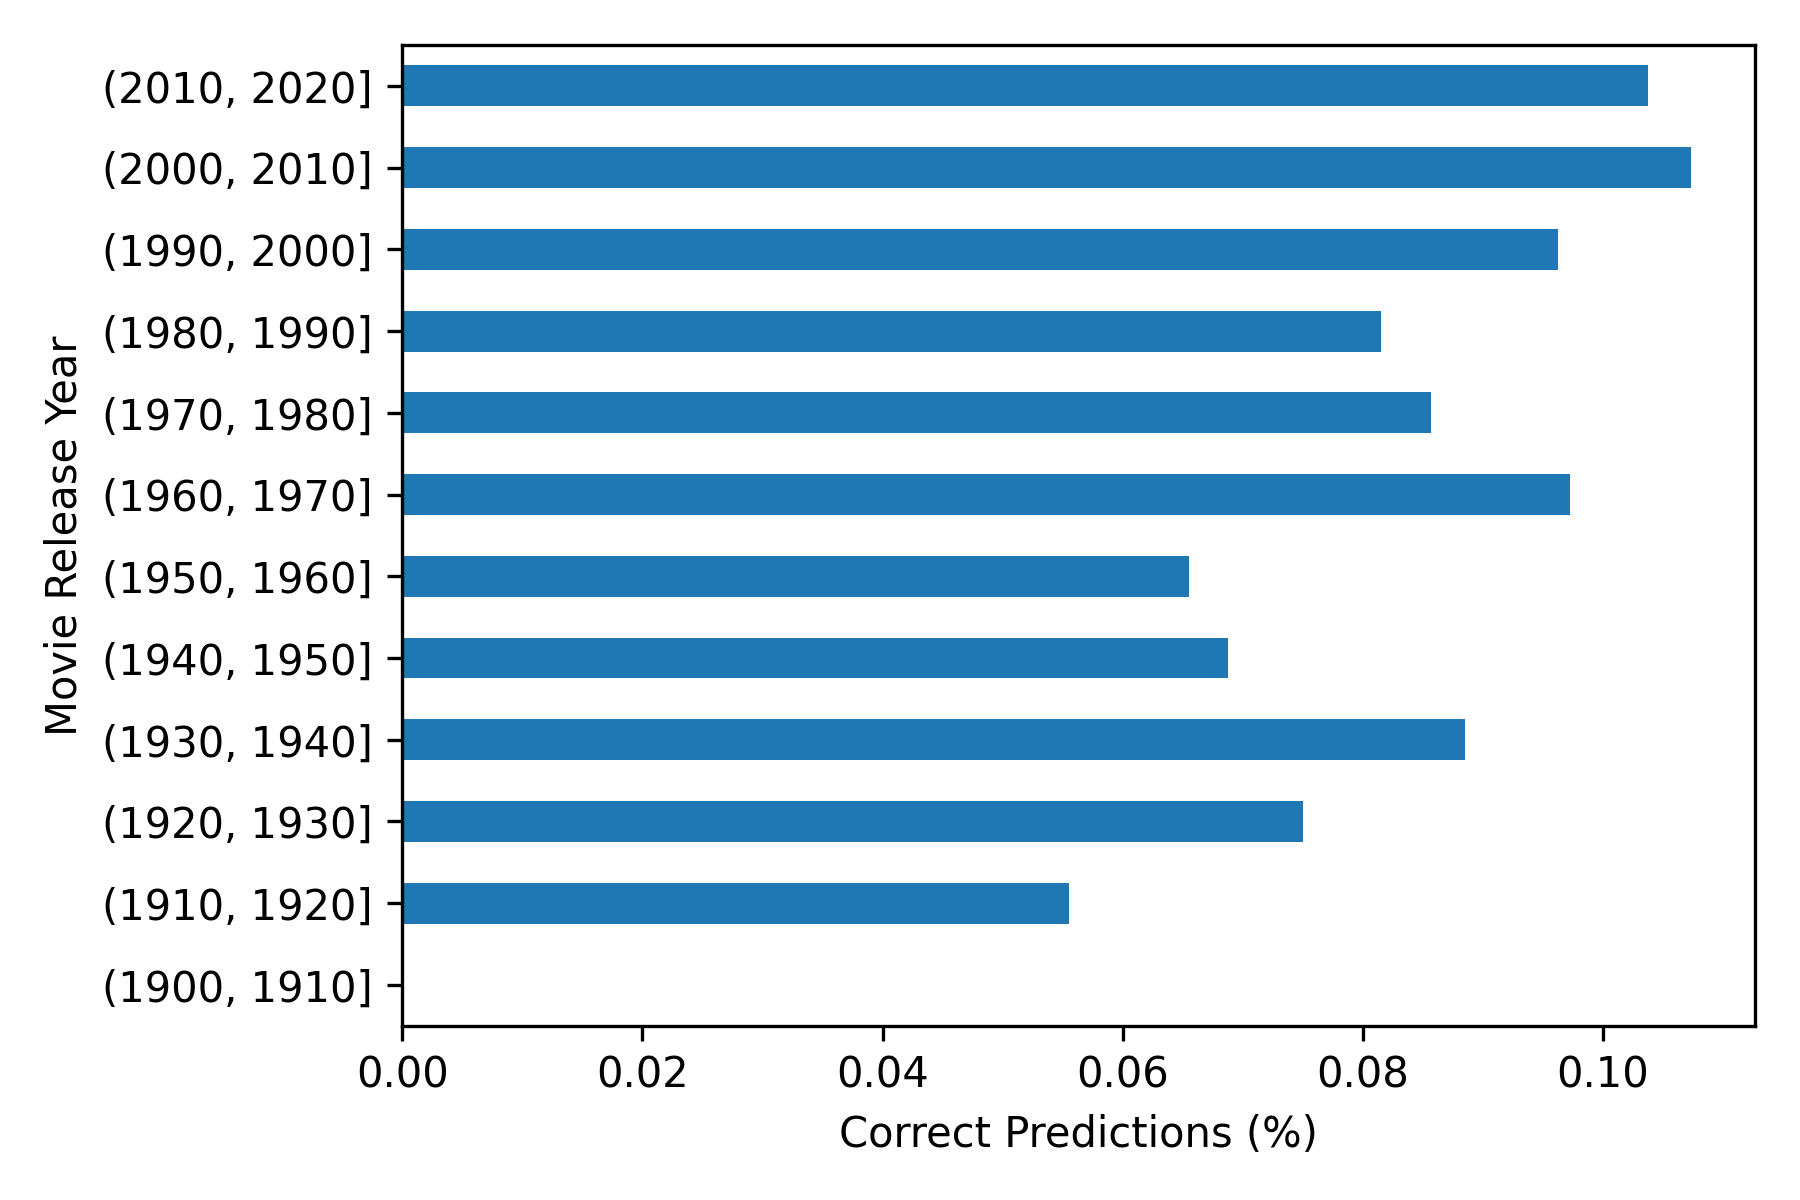
\includegraphics[width=0.4\textwidth]{images/yearlyPrediction.png}
    \caption{Prediction Accuracy across movie years.}
    \label{fig:yearlyPrediction}
\end{figure}

We also examine the impact of age of the movie on the model performance. For example, one can  hypothesize that science fiction movies of a bygone era could be classified into an adventure movie of this era. However, we only observe a marginal increase in accurate predictions from $4\%$ to $6\%$ (Figure~\ref{fig:yearlyPrediction}), that renders age of the movie to be an insignificant factor. 

\subsubsection{Prediction Examples}
We look at a few examples where the models had successes and difficulties in their predictions. We first discuss the positive outcomes for the BERT baseline model. Consider the plot summary for the movie \textit{"High Flying Bird"},

\begin{Verbatim}[fontsize=\small]
    "In the midst of a pro basketball 
    lockout, sports agent Ray 
    Burke (Andre Holland) 
    finds himself caught in the 
    face-off between the league and
    the players. His career is on
    the line,  but Ray is playing 
    for higher stakes. With only 72
    hours to pull off a daring plan, 
    he outmaneuvers all the 
    power-players as he uncovers 
    a loophole that could change 
    the game forever. The outcome 
    raises questions of who owns 
    the game - and who ought to."
\end{Verbatim}

\begin{figure}[!h]
    \centering
    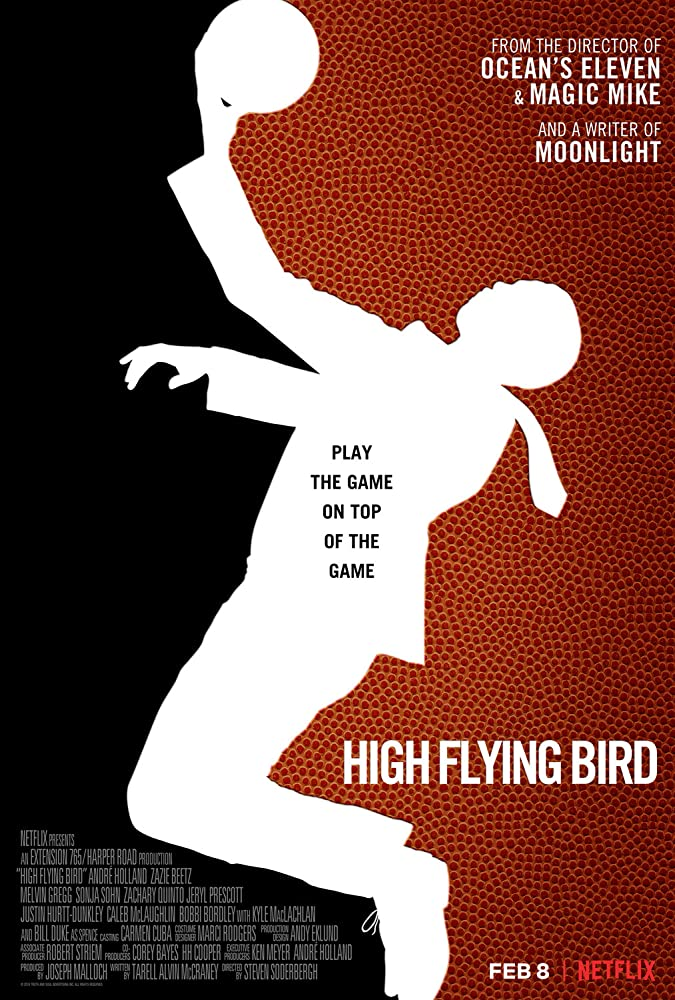
\includegraphics[scale=0.1]{images/HighFlyingBird.jpg}
    \caption{Poster for "High Flying Bird".}
    \label{fig:HighFlyingBird}
\end{figure}

The baseline BERT model with fine-tuning rightly predicts \textbf{Drama}. However, the integrated model predicts \textbf{Crime}. We attribute this prediction error to the features contained within the poster (see Figure~\ref{fig:HighFlyingBird}). The poster is akin to train examples of crime, where many of the posters depict a red color for blood.

Alternately, consider the plot summary for the movie \textit{"All Things To All Men"}. In this case, the baseline BERT fine-tuned model predicts no genre, i.e., a genre not amongst the shortlisted ones (see Section~\ref{sec:DataExploration}). This is a bit surprising since the plot summary, though short in length, seems to clearly indicate a movie with Action and Crime. Interestingly, the integrated model captures the right genres of \textbf{Action} and \textbf{Crime}. The poster for this movie (Figure~\ref{fig:AllThingsToAllMen}) exhibits distinct features that may have aided in its predictions.  
\begin{Verbatim}[fontsize=\small]
    "A thief is caught up in a deadly 
    game of cat-and-mouse between a 
    maverick cop and London crime boss."
\end{Verbatim}

\begin{figure}[!h]
    \centering
    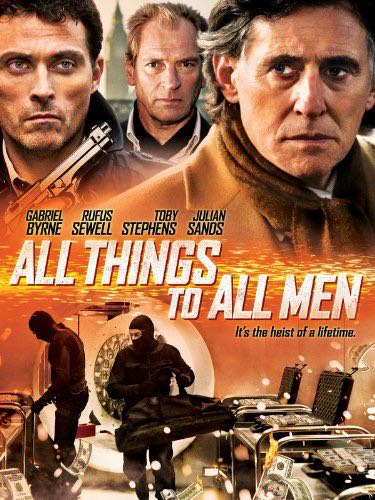
\includegraphics[scale=0.2]{images/AllThingsToAllMen2.jpg}
    \caption{Poster for "All Things To All Men".}
    \label{fig:AllThingsToAllMen}
\end{figure}

We also encounter situations where the ground truth labeling is possibly wrong. For example, the plot summary (\textit{"We are Monster"}) seems to suggest elements of Thriller, Crime and Horror. However, the ground truth label is \textbf{Drama}. Note that the integrated model predicts \textbf{Drama} as well, likely caused by lack of interesting features in the movie poster (Figure~\ref{fig:WeAreMonster}).

\begin{Verbatim}[fontsize=\small]
    "On 8th February 2000 at Feltham Young 
    Offenders Institute, Robert Stewart, 
    a known violent racist was placed 
    in a cell with Zahid Mubarek, a 
    young Asian man due to be released 
    in 6 weeks who had only been convicted
    of petty theft. Over this six 
    week period, Stewart, with his 
    unbalanced mind and deep seated 
    racist tendencies is allowed, 
    through indifference bordering on 
    institutional culpability, to become 
    the ‘monster’ he always wanted to be. 
    Hours before Mubarek’s release, 
    Stewart murdered him in an unprovoked 
    attack."
\end{Verbatim}
\begin{figure}[!h]
    \centering
    
\includegraphics[scale=0.1]{images/WeAreMonster.jpg}
    \caption{Poster for "We are Monster".}
    \label{fig:WeAreMonster}
\end{figure}

% Section : Summary
\section{Conclusion}
In this study, we successfully demonstrate the combined use of movie posters and plot summaries for genre classification. This novel model out-performs state-of-the-art NLP (BERT) models by $2\%$ and shows promise in the classification of minority classes. Although oversampling helps address the data imbalance, it does not completely eliminate it. A larger train dataset will likely mitigate this issue.
We believe further improvements to the poster CNN model will likely improve overall model results. In particular, fine-tuning ResNet models together with BERT will be beneficial. In addition, the use of object detection models~\cite{ChuGuo2017} to identify genre-specific objects such as guns and knives can result in better model performance. On the other hand, it may also be useful to evaluate other language models such as Universal Sentence Encoders~\cite{Cer2018} or bi-directional language models~\cite{Peters2018}.

% Section : Acknowledgements
\section*{Acknowledgements}
We would like to thank our instructors Daniel Cer and Mike Tamir for providing valuable guidance through the course of this work.

% Section : References
%\newpage
\bibliography{w266}
\bibliographystyle{acl}

% Section : Appendix
%\newpage
\onecolumn
\appendix
\label{app:examples}
\section{Examples of Predictions}
% Table~\ref{ErrorAnalysisTable} lists examples of the genre predictions for the BERT and Integrated models. 

\begin{table}[!h]
\small
\begin{center}
\begin{tabular}{|p{2cm}|p{2.5cm}|p{5cm}|p{1.5cm}|p{1.5cm}|}
    \hline 
        \vspace{0.2cm} \bf Movie Name \vspace{0.2cm} & \vspace{0.2cm} \bf Poster & \vspace{0.2cm} \bf Plot Summary & \vspace{0.2cm} \bf Pred. Genre(s) & \vspace{0.2cm} \bf Actual Genre(s)  \\
    \hline
    \vspace{0.2cm}
        Noble Things & 
     \raisebox{-\totalheight}{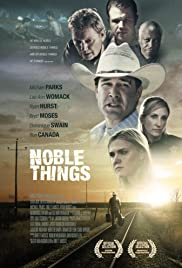
\includegraphics[scale=0.3]{images/NobleThings.jpg}}  \vspace{0.2cm} & \vspace{0.2cm} 
        Jimmy Wayne Collins finds himself adrift in Memphis, Tennessee. Forced to return home to the piney woods of Southeast Texas, Jimmy will face his imprisoned brother, his dying father and the demons he left behind. \vspace{0.2cm} & \vspace{0.2cm} \underline{BERT} \newline None \newline \newline \underline{Integrated} \newline \textbf{Drama} \vspace{0.2cm} & \vspace{0.2cm} Drama \\

    \hline
    \vspace{0.2cm}
        Out of the Past \vspace{0.2cm} & \raisebox{-\totalheight}{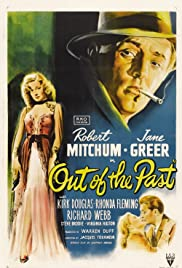
\includegraphics[scale=0.3]{images/OutOfThePast.jpg}}  &  \vspace{0.2cm}
        In a small town in California, the mysterious Jeff Bailey owns a small gas station and is in love with the local Ann. When a stranger just arrived in town meets him, Jeff is ordered to travel to meet the powerful criminal Whit Sterling. Before traveling, Jeff calls Ann and tells her the … \vspace{0.2cm} & \vspace{0.2cm} \underline{BERT} \newline \textbf{Thriller}, Action, \textbf{Crime}, Horror, Adventure, Mystery, Sci-Fi \newline \newline \underline{Integrated} \newline None \newline & \vspace{0.2cm} Drama, Thriller. Crime, Romance \\
        
    \hline
    \vspace{0.2cm}
     Under the Cherry Moon & \raisebox{-\totalheight}{
\includegraphics[scale=0.3]{images/UnderTheCherryMoon.jpg}} & \vspace{0.2cm} 
        Two cousins from Miami, Florida are in the Mediterranean, enjoying life by scamming money off of rich women. One day, they read about a young woman, Mary Sharon (Dame Kristin Scott Thomas), set to inherit fifty million dollars from her father. At first, Tricky (Jerome Benton) has Christopher Tracy (Prince) talked... &  \vspace{0.2cm} \underline{BERT} \newline \textbf{Drama, Comedy, Romance} \newline \newline \underline{Integrated} \newline \textbf{Drama, Comedy, Romance} \vspace{0.2cm} & \vspace{0.2cm} Drama, Comedy, Romance \\
    \hline
    
    \vspace{0.2cm}
     It's Complicated & 
     \raisebox{-\totalheight}{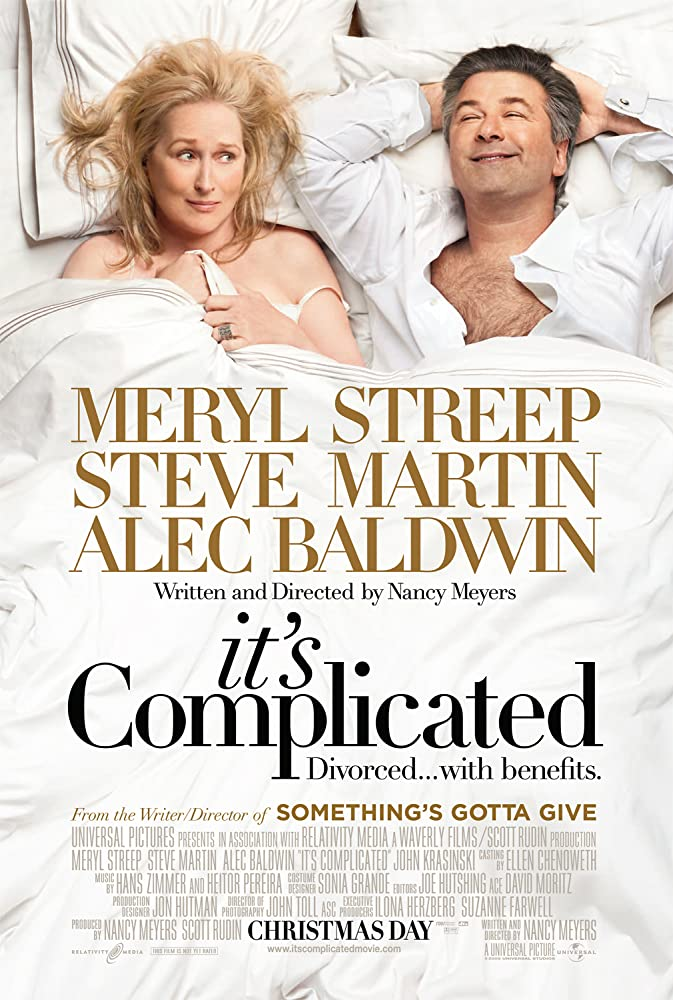
\includegraphics[scale=0.08]{images/ItsComplicated.jpg}} & \vspace{0.2cm} 
        When brought together at a family event, two exes find themselves oddly attracted to each other after ten years of divorce. Although the couple think that this affair will stay in a different state, it brings itself back to their own city and disrupts their personal lives. While the couple still maintain other romances, they cannot help but to continue with their affair. \vspace{0.2cm} &  \vspace{0.2cm} \underline{BERT} \newline \textbf{Drama} \newline \newline \underline{Integrated} \newline \textbf{Drama, Comedy, Romance} & \vspace{0.2cm} Drama, Comedy, Romance \\
    \hline
    
    \vspace{0.2cm}
     Sivas & 
     \raisebox{-\totalheight}{
\includegraphics[scale=0.12]{images/Sivas.jpg}} & \vspace{0.2cm} 
        An eleven-year-old boy and a weathered fighting dog develop a strong relationship after the boy finds the dog wounded in a ditch, left to die. &  \vspace{0.2cm} \underline{BERT} \newline Thriller, Action, Crime, Horror \newline \newline \underline{Integrated} \newline \textbf{Drama} \vspace{0.2cm} & \vspace{0.2cm} Drama \\
    \hline
    
\end{tabular}
\end{center}
\captionsetup{justification=centering}
\caption{\label{ErrorAnalysisTable} Comparison of genre predictions }
\end{table}
\end{document}

% =============================================================================== %
